%FILL IN THE RIGHT INFO.
%\lecture{**LECTURE-NUMBER**}{**DATE**}
\unchapter{Lecture 11}
\lecture{11}{October 8}
\setcounter{section}{0}
\setcounter{theorem}{0}

% **** YOUR NOTES GO HERE:



\section{Meromorphic Functions}

We start by giving an examples of meromorphic functions (defined at the end of last class).

\begin{example}[Meromorphic Functions]
\hphantom{M} %for formatting
\begin{enumerate}
    \item Anything that we have already seen with a pole.
    \begin{center}
        e.g. $\frac{1}{z}$, $\frac{1}{z^2}$, $\frac{1}{z^2+1}$, $\frac{1}{(z-5)^3}$, $\cdots$
    \end{center}
    
    \item Rational functions (a ratio of two finite polynomials)
    \begin{center}
        e.g. $\frac{z}{z^2+1}$, $\frac{1+z+z^2}{(z-1)^2}$, $\frac{z-4}{z+5}$, $\cdots$
    \end{center}
    
    \item Ratio of two holomorphic functions (with denominator $\not\equiv 0$)
    \begin{center}
        e.g. $\frac{e^z}{z^2+1}$, $\frac{z^5+2}{\cos(z)}$, $\cdots$
    \end{center}
\end{enumerate}

\end{example}

\begin{note}
Case 2 follows from case 3 as a special case. We will now prove case 3.
\end{note}

\begin{proposition}
The ratio of two holomorphic functions $\frac{f(z)}{g(z)}$, with $g(z) \not\equiv 0$, is a meromorphic function.
\end{proposition}

\begin{proof}
$f,g$ holomorphic. Thus $\frac{f(z)}{g(z)}$ is holomorphic at all $z$ s.t. $g(z) = 0$. The zeroes of $g$ are isolated. Let $z_0$ be a point where $g$ vanishes. Let $N \geq 1$ be the order of vanishing of $g$ at $z_0$. If $f\equiv 0$ we are done. Thus there are three cases to consider:

\begin{enumerate}
    \item \fbox{$f(z_0) \neq 0$}:
    
    Then we can consider the reciprocal $\frac{g(z)}{f(z)}$. This is non-zero in $\DrP{r}{z_0}$ for some $r>0$. This new function has a zero of order $N$ at $z_0$. By definition, $\frac{f(z)}{g(z)}$ has a pole at $z_0$ of order $N$.
    
    \item \fbox{$f(z_0) = 0$ with order $M<N$}:
    
    Then we write $f(z) = h_1(z) \cdot (z-z_0)^M$ and $g(z) = h_2(z) \cdot (z-z_0)^N$ near $z_0$ with $h_1,h_2$ holomorphic on $D_r(z_0)$. Then $\frac{f(z)}{g(z)} = \frac{h_1(z) \cdot (z-z_0)^M}{h_2(z) \cdot (z-z_0)^N} = \frac{h_1(z)}{h_2(z)} \cdot \frac{1}{(z-z_0)^{N-M}}$, which is a pole of order $N-M$.
    
    \item \fbox{$f(z_0) = 0$ with order $M\geq N$}:
    
    Then, following exactly from case 2, we write $\frac{f(z)}{g(z)} = \frac{h_1(z)}{h_2(z)} \cdot (z-z_0)^{M-N}$, which is holomorphic at $z_0$ with a removable singularity.
    
\end{enumerate}


Thus $\frac{f(z)}{g(z)}$ is meromorphic with every pole being a zero of $g(z)$.
\end{proof}

\begin{note}
    This is the most general formulation of a meromorphic function.
\end{note}

\section{Point at Infinity}

Consider $\C$. $\C$ is not compact, but we can add a single point (our so called ``$\infty$") and define a topology on $\C \cup \set{ \infty }$ such that it is compact.


\begin{definition}[Neighborhood of $\infty$]
A \textbf{neighborhood of $\infty$} is a set $U \subset \C$ open such that $\set{\abs{z} > R} \subset U$ for some $R > 0$
\end{definition}


%[view top right]
\begin{center}

\begin{tikzpicture}


    \draw (0, 3.5, 0) node {$\times$};
    \draw [below right] (0, 3.5, 0) node {$\infty$};
    
    \draw [black][pattern=north west lines] [dotted]
      (-5, 0, -3) -- (-5, 0, 3)
      -- (5, 0, 3) -- (5, 0, -3)
      -- cycle;

    \draw [fill=white] (0, 0, 0) [y={(0,0,1)}] circle (1.5);
    \draw (0,0,0) -- (0,0,1.5);
    \draw [right] (0,0,1.5/2) node {$R$};
    \draw [below right] (5, 0, 0) node {$\C$};
    \draw[->] (3, 1.5, -2) to [out=240,in=120] (3, 0, -2);
    \draw [above] (3, 1.5, -2) node {$\abs{z}>R$};
    
    \draw [fill] (0,0) circle [radius=0.04];
    \draw [above left] (0,0) node {$0$};
    %\draw [color=red][pattern=north west lines][dotted][thick]  (0,0) circle (1.4);
        
     %   \draw [color=red][fill=white][dotted][thick] (50:0.7) circle (0.4);
  \end{tikzpicture}

    
\end{center}




\begin{center}
    $\Downarrow$
\end{center}





\begin{center}
    
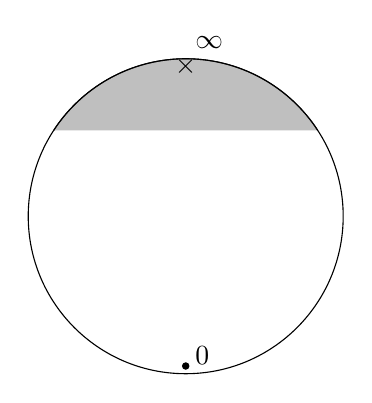
\begin{tikzpicture} % MERC

\def\angEl{18} % elevation angle. Change this for a different angle. DONT CHANGE ANYTHING ELSE UNLESS YOU HAVE OVER 500IQ

\pgfmathsetmacro\H{2*cos(\angEl)}

\fill[white] (0,0) circle (2); % just a white circle

\draw (0,0) circle (2);

\draw[fill=gray,fill opacity=0.5] (0,0,0) ++(33:2cm) arc (33:180-33:2);
\DrawLatitudeCircleF[2]{33}
\DrawLatitudeCircle[2]{0} % equator
\draw (0,\H) node {$\times$};
\draw [above right] (0, \H+0.1) node {$\infty$};

\draw [fill] (0,-\H) circle [radius=0.04];
\draw [above right] (0, -\H-0.1) node {$0$};


\end{tikzpicture}

\end{center}



























If $f:U \to \C$ holomorphic where U is a neighborhood of $\infty$, we can consider $F(z) = \frac{1}{f(z)}$, a holomorphic function on $\set{\abs{z} < \frac{1}{R}} \setminus \{ 0 \}$, a punctured neighborhood around $0$. This set is obtained by taking the reciprocal of $\abs{z}$ in the above definition on $U$. Thus switching $z$ with $\frac{1}{z}$ in some way swaps $\infty$ with $0$.

\begin{definition}
Consider a function $f(z)$ and the function $F(z) = f(\frac{1}{z})$. We say that:
\begin{itemize}
    \item $f$ is \textbf{holomorphic at $\infty$} if $F$ has a removable singularity at $0$.
    \item $f$ has a \textbf{pole of order $N$ at $\infty$} if $F$ has a pole at $0$ of order $N$.
    \item $f$ has an \textbf{essential singularity at $\infty$} if $F$ has an essential singularity at $0$.
    \item $f$ meromorphic on $U$ is \textbf{meromorphic at $\infty$} if $f$ does not have an essential singularity at $\infty$.
\end{itemize}
\end{definition}


\begin{example}
It is easy to get lost in the definition of $F$; take care not to.
\begin{itemize}
    \item $e^{\frac{1}{z}}$, which has an essential singularity at $0$, is holomorphic at $\infty$. This is because $F(z) = e^z$ is holomorphic at $0$.
    
    \item $z^2$, and entire holomorphic function, has a pole at $\infty$ of order 2. This is because $F(z) = \frac{1}{z^2}$ has a pole of order $2$ at $0$.
    
    \item $e^z$ has an essential singularity at $\infty$.
\end{itemize}
\end{example}

\isubsection{THM:Characterization of Rational Functions}

\begin{theorem}[Characterization of Rational Functions]\label{thm:char-rat}

Suppose $f $ meromorphic on $\C$ and $f $ meromorphic at $\infty$. 
Then $f$ is a rational function ($f(z) = \frac{P(z)}{Q(z)}, \, P,Q \in \C [z], \, Q \nequiv 0$).
\end{theorem}

\begin{note}
This theorem means that we can classify meromorphic functions as rational iff they are meromorphic at $\infty$. This is significant since the set of polynomials is much smaller than the set of all meromorphic functions. This also implies that almost all meromorphic functions will have an essential singularity at $\infty$ (since few are rational, and all others must have an essential singularity at $\infty$).
\end{note}

\begin{proof}[\ref{thm:char-rat}]
Let $f$ meromorphic on $\C$. Then the poles of $f$ do not accumulate in $\C$. The poles of $f$ cannot accumulate at $\infty$ since $f$ is meromorphic at $\infty$ (since $f(\frac{1}{z})$ has a pole or removable singularity at $0$, it will be holomorphic and non-zero in $\DrP{r}{0}$ for some $r>0$, so $f$ has no poles in some punctured neighborhood of $\infty$). 

It follows that since they cannot accumulate anywhere, $f$ has finite poles $\set{z_1, \cdots ,z_n}$ (and possibly $\infty$). Let $z_k$ be a pole in $\C$. Write for $z$ near $z_k$:
\begin{align*}
    f(z) = \underbrace{f_k(z)}_{principal} + \underbrace{g_k(z)}_{hol'c}
\end{align*}
with $g_k(z)$ a polynomial in $\frac{1}{z-z_k}$. We do the same at $\infty$:
\begin{align*}
    f \left( \frac{1}{z} \right) = \underbrace{\Tilde{f}_\infty(z)}_{principal} + \underbrace{\Tilde{g}_\infty(z)}_{hol'c}.
\end{align*}

Note that $\Tilde{f}_\infty(z)$ could be equal to $0$ if there is no pole at $\infty$. Note further that $\Tilde{g}_\infty(z)$ is holomorphic in a neighborhood of $0$.

Let $f_\infty(z) = \Tilde{f}_\infty\left( \frac{1}{z} \right)$. Since $\Tilde{f}_\infty$ is a polynomial in $\frac{1}{z}$, $f_\infty$ is a polynomial in $z$. Let:
\begin{align*}
    H(z) = f(z) - f_\infty(z) - \sum_{k=1}^n f_k(z).
\end{align*}
 $H$ is a holomorphic function on $\C \setminus \bigcup_{k=1}^n \{z_k \}$. Near $z_k$ we have that $f_\infty$ is bounded (as it is a polynomial), that $f-f_k$ is bounded (since it is equal to $g_k$, a holomorphic function), and that $f_i$ (for $i \neq k$) is bounded. Thus $H$ is bounded near $z_k$. Near $\infty$ we have: 
\begin{align*}
H\left( \frac{1}{z} \right) &= f\left( \frac{1}{z} \right) - f_\infty\left( \frac{1}{z} \right) - \sum_{k=1}^n f_k\left( \frac{1}{z} \right)\\
\text{($P(x) \vcentcolon = $ ``a polynomial in x") } &=\underbrace{f\left( \frac{1}{z} \right) - \Tilde{f}_\infty\left( z \right)}_{\Tilde{g}_\infty (z)} - \sum_{k=1}^n P_k\left( \frac{1}{\frac{1}{z} - z_k} \right).
\end{align*}
Both of these are bounded since $\Tilde{g}_\infty$ is bounded for $z$ close to $0$ and $\left( \frac{1}{\frac{1}{z} - z_k} \right) \xrightarrow[]{z \to 0} 0$ (hence the rightmost sum of polynomials is bounded). Thus $H$ is bounded in a neighborhood of $\infty$ and bounded in some union of neighborhoods $\bigcup_{j=1}^n \DrP{r}{z_j}$. But $H$ is holomorphic (and thus bounded) on the complement of these neighborhoods (since $H$ is meromorphic with all possible poles caught by our neighborhoods). $H$ is thus bounded on $\C$. By corollary (\ref{cor:liouville}), $H(z) = c \in \C$ is constant. Thus:
\begin{align*}
    f = \underbrace{\sum_{k=1}^n f_k}_{rational} + \underbrace{f_\infty +c}_{polynomial}
\end{align*}

Thus $f$ is a rational function.
\end{proof}


\section{Argument Principle/Logarithmic Derivative Formula}

The main usefulness of meromorphic functions is their applicability to this following theorem:

\isubsection{THM: Argument Principle}

\begin{theorem}[Argument Principle]\label{thm:arg-princ}

$f$ meromorphic on $\oic$ open, $\om ' \ssubset \om$ open subset with piecewise smooth boundary. Suppose that $f$ has no zeroes and no poles on $\partial \om '$. Then:
\begin{align*}
    \frac{1}{2 \pi i} \int_{\partial \om '} \frac{f'(z)}{f(z)} \dif z \;\; = \;\;\; & \# \set{\text{zeroes of $f$ in $\om '$ (with multiplicities)  } }\\
    -  &\# \set{ \text{ poles of $f$ in $\om '$ (with multiplicities) } }.
\end{align*}

\end{theorem}

\begin{note}
$\left( \frac{f'}{f} \right)$ is called the logarithmic derivative, naively ``$(log(f))'$" . ``With multiplicities" means that a zero/pole of order $N$ counts like $N$.
\end{note}

\begin{center}
\begin{tikzpicture}
    \draw[shift={(-2.5,-2.5)},rotate=0][dotted][scale =2.5] plot [smooth cycle] coordinates {(0,0) (1,0.1) (2,0.3) (2,0.7) (1.5,1.5) (0.8,1.5) (0.3,1.2) (-0.2,0.6) };
    \draw [below left] (-2.45,-2.45) node {$\Omega '$};
    
    \draw (0,0.3) node {$\times$};
    \draw [fill] (1,0.5) circle [radius=0.04];
    \draw (-2,-1) node {$\times$};
    \draw [fill] (-1,-1.5) circle [radius=0.04];
    \draw (1,-1.5) node {$\times$};
    \draw [fill] (-1.2,-0.4) circle [radius=0.04];
    
    
\end{tikzpicture}    
\end{center}



\begin{proof}[\ref{thm:arg-princ}] Let us investigate the behaviour of $\left( \frac{f'}{f} \right)$. Let $z_0$ be either a zero of order $N$ or a pole of order $-N$ of $f$ inside $\om '$. We want to expand in a Laurent series; $f(z) = \sum_{n=N}^\infty a_n (z-z_0)^n$ with $a_N,N \neq 0$.

We can write $f(z)  = (z-z_0)^N \cdot g(z)$ for $z$ near $z_0$ where $g$ is holomorphic and non-zero in a neighborhood of $z_0$. Thus on $\DrP{r}{z_0}$:
\begin{align*}
\frac{f'(z)}{f(z)} &= \frac{N(z-z_0)^{N-1} g(z) + (z-z_0)^N g'(z)}{(z-z_0)^N g(z)}\\
&= \frac{N}{z-z_0}+ \frac{g'(z)}{g(z)}.
\end{align*}

The second term is holomorphic. The first term is a simple pole with residue $N$. Thus $\res{z_0}{\frac{f'}{f}} = N$. The same computation on $\frac{g'(z)}{g(z)}$ yields a similar equation, but with $N=0$, indicating that there are no poles along the boundary. Applying theorem (\ref{thm:residue-formula}) gives us:
\begin{align*}
    \frac{1}{2 \pi i} \int_{\partial \om '} \frac{f'(z)}{f(z)} \dif z = \sum_{z_i \in S} \res{z_0}{\frac{f'}{f}} = \sum_{zeroes} 1 - \sum_{poles} 1.
\end{align*}
where $S$ is the set of all poles of $\frac{f'}{f}$ in $\om '$. This is the same as the set of all zeroes and poles of $f$.

\end{proof}


\isubsection{THM: Rouché}

\begin{theorem}[Rouché]\label{thm:rouche}

$f,g$ holomorphic on $\om$, $\om' \ssubset \om$, $\om ' $ piecewise smooth boundary. Suppose that $\abs{f(z)} > \abs{g(z)} \, \forall z \in \partial \om '$. Then $f $ and $f+g$ have the same number of zeroes in $\om ' $ (counted with multiplicities).

\end{theorem}

\begin{note}

The logic of this theorem is that $g$ is some kind of perturbation such that on the boundary $g$ has less effect than $f$. Then the number of zeroes does not change.

\end{note}

\begin{proof}[\ref{thm:rouche}] Use a ``homotopy argument".

Connect $f$ and $f+g$ via $f_t(z) = f(z) + tg(z), \, t \in [0,1]$. Then $f_t$ holomorphic on $\om \, \forall t$. Let $n_t = \# \set{ \text{zeroes of $f_t$ inside $\om '$  }}$ (we want to show that $n_0 = n_1$). We shall show that $n_t$ is constant in $t$ by applying theorem (\ref{thm:arg-princ}). To apply it, we must have that $f $ has no zeroes on the boundary (it has no poles since it is holomorphic). Then for $z \in \partial \om '$:
\begin{align*}
    \abs{f_t(z)} = \abs{f(z) + tg(z)} &\geq \abs{f(z)} - t\abs{g(z)}\\
    \text{(since $t\in [0,1] $) }&\geq \abs{f(z)} - \abs{g(z)}\\
    \text{(apply assumption) }&> 0.
\end{align*}

Thus $f_t$ has no zeroes on the boundary, so:
\begin{align*}
    n_t = \frac{1}{2 \pi i} \int_{\partial \om '} \frac{f'(z)}{f(z)} \dif z.
\end{align*}

Now note that $f_t$ is a $C^0$ function in both $z$ and $t$. Thus the contour integral in $z$ is a $C^0 $ function of $t$. It follows that the map $[0,1] \to \mathbb{Z}, \, t \mapsto n_t$ is continuous. Since $\mathbb{Z}$ is disconnected, $n_t$ must be constant.


\end{proof}












































